
%----------------------------------------------------------------------------------------
%	PACKAGES AND OTHER DOCUMENT CONFIGURATIONS
%----------------------------------------------------------------------------------------

\documentclass{article}

\usepackage{fancyhdr} % Required for custom headers
\usepackage{lastpage} % Required to determine the last page for the footer
\usepackage{extramarks} % Required for headers and footers
\usepackage{graphicx} % Required to insert images
\usepackage{mathtools, bm}
\usepackage{amssymb, bm}
\usepackage{graphicx}
\usepackage{algorithmic}

% Margins
\topmargin=-0.45in
\evensidemargin=0in
\oddsidemargin=0in
\textwidth=6.5in
\textheight=9.0in
\headsep=0.25in


\linespread{1.1} % Line spacing

% Set up the header and footer
\pagestyle{fancy}
\lhead{\hmwkAuthorName} % Top left header
\chead{\hmwkClass\ (\hmwkClassInstructor\ \hmwkClassTime): \hmwkTitle} % Top center header
\rhead{\firstxmark} % Top right header
\lfoot{\lastxmark} % Bottom left footer
\cfoot{} % Bottom center footer
\rfoot{Page\ \thepage\ of\ \pageref{LastPage}} % Bottom right footer
\renewcommand\headrulewidth{0.4pt} % Size of the header rule
\renewcommand\footrulewidth{0.4pt} % Size of the footer rule

\setlength\parindent{0pt} % Removes all indentation from paragraphs

%----------------------------------------------------------------------------------------
%	DOCUMENT STRUCTURE COMMANDS
%	Skip this unless you know what you're doing
%----------------------------------------------------------------------------------------

% Header and footer for when a page split occurs within a problem environment


% Header and footer for when a page split occurs between problem environments
   
%----------------------------------------------------------------------------------------
%	NAME AND CLASS SECTION
%----------------------------------------------------------------------------------------
\newcommand{\logoepfl}{
  \begin{center}
    
\includegraphics[width=4cm]{img/epfl.jpg}
  \end{center}
  \vspace{0.3cm}
  \hrule
}


\newcommand{\hmwkTitle}{Decentralized Data Sharing System based on Secure Multiparty Computation} % Assignment title
\newcommand{\hmwkDueDate}{Autumn 2017} % Due date
\newcommand{\hmwkClass}{IN, LCA1} % Course/class
\newcommand{\hmwkClassTime}{} % Class/lecture time
\newcommand{\hmwkClassInstructor}{D.Froelicher, J.Troncoso-Pastoriza} % Teacher/lecturer
\newcommand{\hmwkAuthorName}{Max Premi} % Your name

%----------------------------------------------------------------------------------------
%	TITLE PAGE
%----------------------------------------------------------------------------------------
\title{
\logoepfl
\vspace{2in}
\textmd{\textbf{\hmwkClass:\ \hmwkTitle}}\\
\normalsize\vspace{0.1in}\small{Due\ on\ \hmwkDueDate}\\
\vspace{0.1in}\large{\textit{\hmwkClassInstructor\ \hmwkClassTime}}
\author{\textbf{\hmwkAuthorName}}
\vspace{3in}
}

%----------------------------------------------------------------------------------------

\begin{document}

\maketitle

\newpage
\section*{Abstract}
\addcontentsline{toc}{section}{Abstract}
Unlynx and Prio are two privacy-preserving data sharing systems, with each it's way to encode, decode and aggregate datas. While Unlynx uses homomorphic encryption based on Elliptic Curve ElGamal and zero knowledge proofs, Prio uses Secret-sharing encoding and \textit{secret-shared non-interactive proofs}(SNIP's), which is supposed to perform much better than classic zero knowlege proof in term of computation time, by doing a trade-off execution time/bandwidth.\\
We consider $m$ servers that consitute the collective authority whose goal is to verifiably compute aggregation functions over data send by $n$ data providers.\\
Several problems arise when you want to compare Unlynx and Prio. First, server are static in the first one but not in the second, and the threat model are not exactly the same, as you need to trust at least one server in Unlynx, but all in Prio for correctness. Privacy is assured if at least one server is trusted for both sytem. Then, data providers have all their data encrypted, while Prio do not use homomorphic encryption, and do not need to store data at all.\\
Prio also extends classic private aggregation techniques to enable collection of different class of statistics such as least-square regression, as Unlynx System can only compute sum and count querry over data.\\
The goal of this project is to, first implement Prio in the Unlynx framework, second to implement input validation for Unlynx, and then modify both protocol to be ran with the least significant difference in term of assumption and model.\\
Then if possible we want to design a System that implement the best of both sytems. The idea would be to use Prio encoding to do more than just summing and counting, by removing the encryption at the data provider, and doing the computation in local and then transfer to server in an encrypted way.\\
-------------------------------------------------
%	TABLE OF CONTENTS
%----------------------------------------------------------------------------------------

\newpage
\tableofcontents
\newpage


%----------------------------------------------------------------------------------------
%	BEGIN OF REPORT
%----------------------------------------------------------------------------------------

\section*{Introduction}
\addcontentsline{toc}{section}{Introduction}
Nowadays, tons of data are generated around us and about what we do, and are used to compute statistics. Even if these statistics are colleted with the goal of learning usefull aggregate informations about the users/population, it might end in collecting and storing private data from client.\\
The need to collect data and to share them in a privacy-preserving way has become crucial in this context.
We can for example illustrate this with the problem of Cloud leaking that happened several times in the past years.[ref]\\
Leaking private user data bring important privacy and security risks. They might be discloded, sold for profit or even be used by agencies for targeting and mass surveillance goals.\\
A lot of techniques have been developed through the years, by major technology companies such as Google [references], but also researcher in Universities [references].\\
However, by gaining \textit{privacy}, these protocols sacrifice \textit{robustness} and \textit{scalability}, which are two important aspect to keep in mind while designing a decentralized system. Privacy is necessary so that no leak in the sensitive data happend, and robustness characterise the correctness of the computation. The trade-off between both should be reasonable, as we do not want any data to be leaked, and the server has to correctly compute under given circunstunces.
This difficulties lead to the use of technical agreements rather than technical solutions.\\
Indeed, centralized system are still widely used [ref] as they are way simpler and use a trusted third party. But these trusted parties still is a single point of failure in the system and data provider begin to realize the value of their own datas.\\
This is why decentralized sytems are becoming more popular, and desirable.\\
In this paper, we present the implementation of Prio into Unlynx and compare them with input validation proof.

\section*{Contributions}
\section*{Background}

\section{Unlynx System}
\begin{itemize}
\item How does unlynx work (with a figure) (system of client, queries and servers)
\item How Aggregation is done
\item How proof is done
\end{itemize}
\subsection{Model}
Unlynx is a privacy-preserving data sharing system developed by LCA1 in collaboration with DeDiS.\\
It consists of a collective authority (CA) formed by a number $m$ of server $S_1,...S_m$, and $n$ data providers $DP_1,...DP_n$ containing sensitive data. These DPs combined represent a distributed database that is used to awnser queries made by a querier $Q$. The querier and DPs choose one server of the CA to communicate with and can change this choice at any given time.\\
\textbf{Functionality}: Unlynx should permit SQL queries of the form SELECT SUM(*)/COUNT(*) FROM DP,.... WHERE * AND/OR GROUP BY *, with any number of * clauses.\\
\textbf{Privacy and Robustness}: Both are assured if at least one server is trusted, as we use the fact that we are allowed to publish ciphertext and their aggregation to show that the computation at the server are actually correct. It leaks nothing as all data are encrypted.

\subsection{Threats}
\textbf{Collective authority servers} It is assumed an Anytrust model [REF]. It does not requires any particular server to be trusted or to be honest-but-curious. The moment it exists one server that is not malicious, functionality, security and privacy are guaranteed.\\
\textbf{Data providers} are assumed to be honest-but-curious. The system does not protect against malicious DPs sending false infomations, but a solution will be discuss  in Section [INPUT RANGE VALID SECTION].\\
\textbf{Queriers} are assumed to be malicious, and can collude between themselves or with a subset of the CA servers.\\
It is also assumed tha all network communication is encrypted and authenticated, by using a protocol like TLS for example.

\subsection{Pipeline and proof}
The protocol start when a querier wants to retrieve some information about sensitive data. It sends the query to one of the server of the CA. Upon receiving, the server broadcast this query to the other servers in the collective authority.\\
From here the data are privately and securely processed by the CA, before sending back the result to the querier, encrypter over the public key of the Querrier. During all the steps of the protocol, the server will never get the data in clear.\\
The pipeline is the following: Encryption, Verification Shuffle, Distributed Deterministig Tag, Collective Aggregation, Distributed Results Obfuscation, Key Switch. At the end of this pipeline, the querier get the data and can decrypt them to get the aggregate statistics he asked for, without any server seeing the data in clear, or knowing from which data provider the data are from.
\begin{figure}[h]
\centering
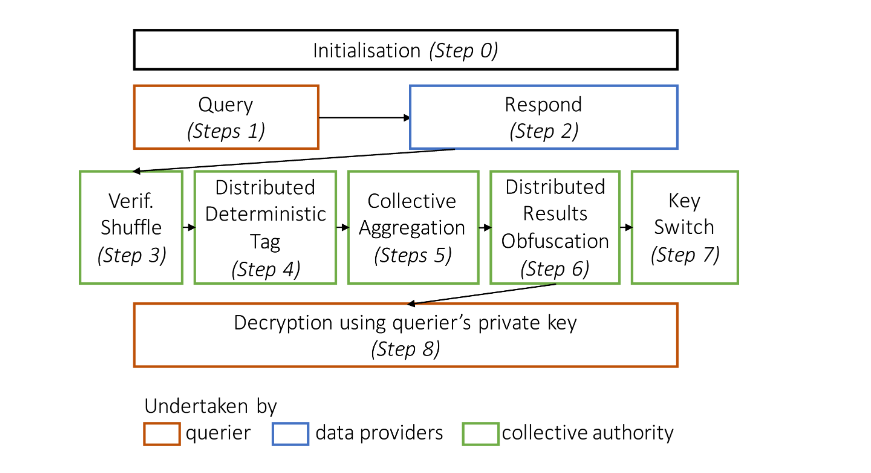
\includegraphics[scale=0.5]{img/unlynxPip.png}
\caption{Unlynx query processing pipeline}
\end{figure}
\\
\textbf{Proofs} are done with zero-knowledge systems, to preserve privacy. There is one for each state of the pipeline, for example when aggregating, it publishes the ciphertexts, and the result of their aggregation, as the data is encrypted using Elliptic curve ElGamal, it leaks nothing about the data alone, but there is no Input range proof , meaning the DPs can send fraudulous data (by giving a very big number, and as it is encoded we cannot verify it) and make the computation wrong. This input validation proof is implemented and described in section [SECTION]\\

\subsection{Input range validation for ElGamal}

rnoiuezbfnoizenbfoieznofezifnezoin


\section{Prio System}
\begin{itemize}
\item How does Prio work (same as before)
\item How does Aggregation is done
\item New proof system SNIPs
\end{itemize}
\subsection{Model}
Prio is also a privacy-preserving data sharing system developed Standford University.\\
It consists of a collective authority (CA) formed by a number $m$ of server $S_1,...S_m$,and each data provider holds a private value $x_i$ that is sensitive. 
Unlike Unlynx, Prio do not encrypt private value $x_i$ that why it is a more challenging aggregation in terms of privacy.\\
Communication is assumed to be done in secure channels as previously described.
\textbf{Functionality}: Prio should permit the collective authority to compute some aggregation function $f(x_1,...x_n)$ over private values of data providers, in a way that leaks as little as possible about these, except what can be inferred from the aggregation itself.
\textbf{Privacy and Robustness}: Privacy is assured if at least one server is trusted, but robustness is satisfied if and only if all server are trusted, as you cannot be assured that computation at the server are correct.	
\
\subsection{Threats}
Unlynx is a privacy-preserving data sharing system developed by LCA1 in collaboration with DeDiS.\\
It consists of a collective authority (CA) formed by a number $m$ of server $S_1,...S_m$, and $n$ data providers $DP_1,...DP_n$ containing sensitive data. These DPs combined represent a distributed database that is used to awnser queries made by a querier $Q$. The querier and DPs choose one server of the CA to communicate with and can change this choice at any given time.\\
\textbf{Functionality}: Unlynx should permit SQL queries of the form SELECT SUM(*)/COUNT(*) FROM DP,.... WHERE * AND/OR GROUP BY *, with any number of * clauses.\\
\textbf{Privacy and Robustness}: Both are assured if at least one server is trusted, as we use the fact that we are allowed to publish ciphertext and their aggregation to show that the computation at the server are actually correct. It leaks nothing as all data are encrypted.

\subsection{Threats}
\textbf{Collective authority servers} In Prion it is needed that one server is not malicious and trusted, so that security and privacy are guaranteed.\\
Robustness against malicious server seems desirable but doing so would cost privacy and perfomance degradation, which is not desirable.\\
\textbf{Data providers} are assumed to be malicious. The system protects itself against malicious DPs. All data that does not pass the SNIPs proof, will be discarded.\\

\subsection{Pipeline and proof}
do 
\section*{Prio SNIPs}
\begin{itemize}
\item Client evaluation
\item Consistency checking at the server
\item Polynomial identity test
\item Multiplication of shares
\item Output verification

\end{itemize}


\section{Implementation}
 
 
 nziefnoezifoezfzoioezifoezifoizen oirfezifnioznfzoei nzoi nfzioe
\begin{itemize}

\item what is implemented in a little more detailled
\item optimization apported by code from github and not aborded in details

\end{itemize}


\section{Performance evaluation}

Explain a little more about comparison and test settings


\begin{itemize}


\item Scaling with number of server
\item Scaling with number of client
\item Scaling with fairly high number of both 
\item Time and Bandwidth dilemna

\end{itemize}


\section{Comparison Theory and Performance}
Comparison but explaining why it's cannot be perfectlhy matched, because of the differents assumptions.

\section{Future Work}

\newpage
\section*{Conclusion}
iufznfiozfoezizefez fze
fezfezfezfezfezfezf
ezfezfezfzefezfezfezfezfezfzefzefezfezfezfezfezfezfezfz

\newpage
\section*{References}

inoinofizefnoezifnezoifnez

\end{document}
